\documentclass{book}
\usepackage{etex}
\usepackage{geometry}
\geometry{papersize={170mm,240mm},total={140mm,200mm},top=21mm,bindingoffset=10mm}
\usepackage[english,ngerman]{babel}
\usepackage[utf8]{inputenc}
\usepackage[T1]{fontenc}
\usepackage{cancel}
\usepackage{times}
\usepackage{amsmath,amscd}
\usepackage{amssymb}
\usepackage{amsfonts}
\usepackage{amsthm}
\usepackage{graphicx}
\usepackage{fancyhdr}
\usepackage{textcomp}
\usepackage{txfonts}
%\usepackage{alltt} 
\newcommand\hmmax{0}
\newcommand\bmmax{0}
\usepackage{bm}
\usepackage{verbatim}
\usepackage{paralist}
\usepackage{makeidx}
\usepackage{array}
%\usepackage[colorlinks=true]{hyperref}
\usepackage{hyperref}
\usepackage{subfigure}
\usepackage{tikz}
\usepackage{pgfplots}
\usepackage{pgfplotstable}
\usepackage{pdftexcmds}
\usepackage{pgfmath}
%\usepackage{placeins}
%\usepackage{subfigure}
\usepackage[autostyle=false,english=american]{csquotes}
%\usepackage{float}
%\usepackage{enumitem}
\usepackage{wasysym}
\usepackage{environ}
%\usepackage{pifont}
%\usepackage{feynmp}
\usepackage{appendix}
\usetikzlibrary{calc,intersections,through,backgrounds,graphs,positioning,shapes,arrows,fit}
\usetikzlibrary{patterns,decorations.pathreplacing}
\usetikzlibrary{decorations.pathreplacing}
\usetikzlibrary{external}
\usetikzlibrary{datavisualization}
\usepackage[europeanvoltages,
europeancurrents,
europeanresistors,   % rectangular shape
americaninductors,   % "4-bumbs" shape
europeanports,       % rectangular logic ports
siunitx,             % #1<#2>
emptydiodes,
noarrowmos,
smartlabels]         % lables are rotated in a smart way
{circuitikz}          %
\usepackage{siunitx}
\usepackage{tabularx}
\usetikzlibrary{arrows}
\usepackage{algpseudocode}
\usepackage{algorithm}
\usepackage{gensymb}
\usepackage{mathtools}



\tikzstyle{inputNode}=[draw,circle,minimum size=10pt,inner sep=0pt]
\tikzstyle{stateTransition}=[-stealth, thick]


\begin{document}

\begin{figure}
	\centering
	\begin{tabular}{ccc}
		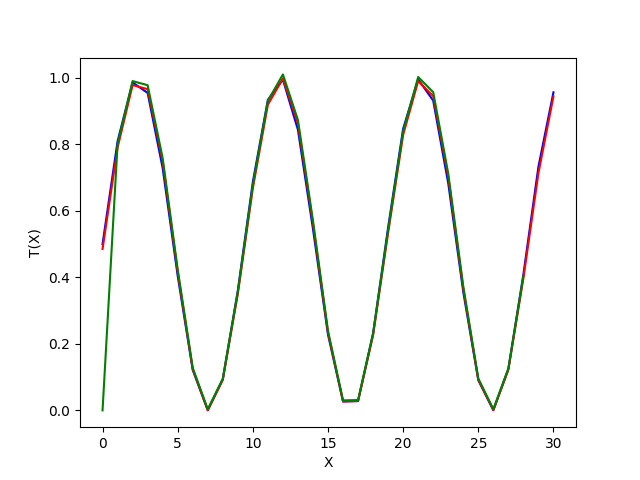
\includegraphics[scale=0.27]{learning/img/burger_predict0.png} &
		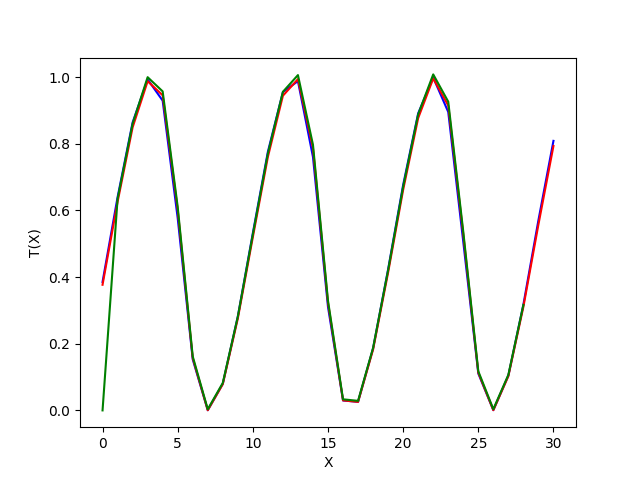
\includegraphics[scale=0.27]{learning/img/burger_predict10.png} &
		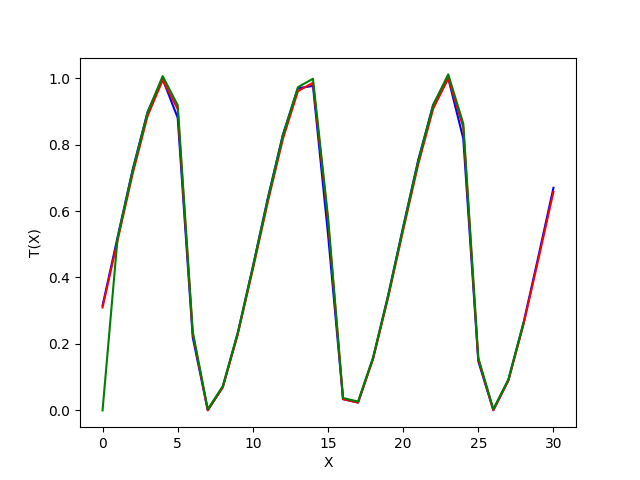
\includegraphics[scale=0.27]{learning/img/burger_predict20.png}
	\end{tabular}
	\label{fig:mst_multiplicator_error}
	\caption{Das vorhersagen des nächsten Zeitschrittes scheint gut zu funktionieren. Blau repräsentiert den aktuellen Zustand $i$, rot den berechneten Zustand $i+1$ und grün den vom neuronalen Netzwerk vorhergesagten Zustand $i+1$. }
\end{figure}

\end{document}